%!TEX root = ../paper.tex

\subsection{Classification}
\label{sec:classification}

After we came up with clusters and cluster labels for all blog posts in a database, we need a method to classify new blog posts. % e.g. so new clustering is not needed for every single blog post
To achieve this we calculate the same features vectors for the single new blog post, as were extracted for the blog posts in the original clustering.
Based on these feature vectors we can now decide to which cluster the blog post belongs.


The first naive idea that came into our mind was to calculate the euclidean distance from the blog post to the center points of the clusters.
The resulting cluster would then be the one with the lowest distance.
While this method is computationally simple and fast, it might not provide the best possible results.
Therefore we looked at more sophisticated approaches that were used for similar problems before.
We applied two of those methods, k-Nearest Neighbor algorithm and a Support Vector Machine [TODO: references?].


\subsubsection{k-Nearest Neighbor}
\label{sec:k_nearest_neighbor}


The k-Nearest Neighbor algorithm selects the number of $k$ vectors which are closest to the feature vector of the new blog post.
Then it returns the cluster that is most common amongst these neighbors as a result. 
For example consider the scenario depicted in Fig.~\ref{fig:naive}.
The naive method of calculating the euclidean distance between the cluster center and the feature vector of the new blog post would have cluster 1 as a result.
However the k-Nearest Neighbor algorithm with, for example $k=5$, returns cluster 2, because 4 out of the 5 closest neighbors belong to cluster 2.
This also seems correct compared to our human intuition, because the feature vector of the new blog post seems to be naturally belonging to cluster two.


\begin{figure}
    \centering
    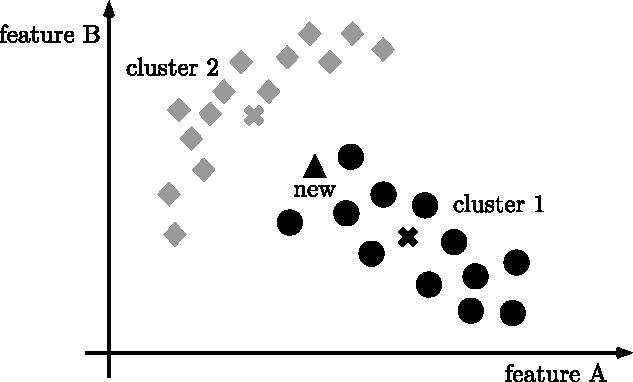
\includegraphics[]{images/naive.pdf}
    \caption{The naive approach, which calculates the euclidean distance to the center of the cluster, would put the new blog post into cluster 1. The k-Nearest Neighbor algorithm would return cluster 2 as a result.}
    \label{fig:naive}
\end{figure}


\subsubsection{Support Vector Machine}
\label{sec:support_vector_machine}


A Support Vector Machine creates a model to distinguish between the different clusters.
(see Fig.~\ref{fig:svm})


\begin{figure}
    \centering
    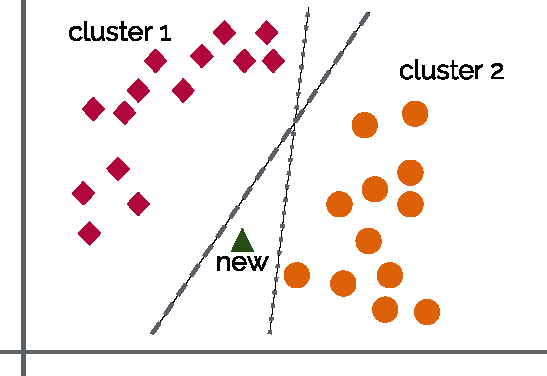
\includegraphics[]{images/svm.pdf}
    \caption{Two differently configured Support Vector Machines might provide the two different lines as borders between the different clusters. The dotted line would result in the blog post belonging to cluster 1, while the dashed line would return cluster 2 as a result.}
    \label{fig:svm}
\end{figure}
